
%%%%%%%%%%%%%%%%%%%%%%%%%%%%%%%%%%%%%%%%%%%%%%%%% Zielsetzung %%%%%%%%%%%%%%%%%%%%%%%%%%%%%%%%%%%%%%%%%%%%%%%%%%%%%

\section*{\LARGE\textbf{Zielsetzung}}

In dem Projekt soll ein neuronales Netz zur Erkennung von Objekten entwickelt werden. Dieses neuronale Netz soll auf verschiedenen Systemen zum Vergleich der Performance genutzt werden. Dabei soll bei der Konzeption und Entwicklung darauf geachtet werden, ein realitätsnahes Beispiel umzusetzen.


%%%%%%%%%%%%%%%%%%%%%%%%%%%%%%%%%%%%%%%%%%%%%%%%% Anwendungsbeispiele %%%%%%%%%%%%%%%%%%%%%%%%%%%%%%%%%%%%%%%%%%%%%%%%%%%%%

\section*{\LARGE\textbf{Anwendungsbeispiele}}

In dem Anwendungsbeispiel soll mit Hilfe eines Fotos eines Tieres dessen Tierart bestimmt werden. 

\begin{figure}[htbp]
	\centering
		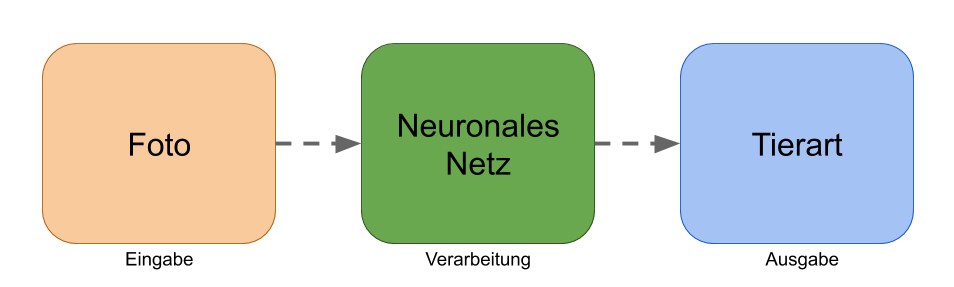
\includegraphics[width=1.00\textwidth]{BilderPDF/zielsetzung/Prinzip.png}
	\label{fig:Prinzip}
\end{figure}

Dies könnte ein realistischer Anwendungsfall für eine App eines Zoos sein. Diese App würde das Foto des Tieres an einen Server senden, welcher die Auswertung des Fotos übernimmt. Anschließend erhält die App die sichtbare Tierart zurück. Auf diese Art wäre es dem Zoo  möglich einen Audio Tour Guide anzubieten. Im Idealfall sogar in der Muttersprache des Besuchers - abhängig davon in welcher Sprache er die App installiert hat. 

\begin{figure}[htbp]
	\centering
		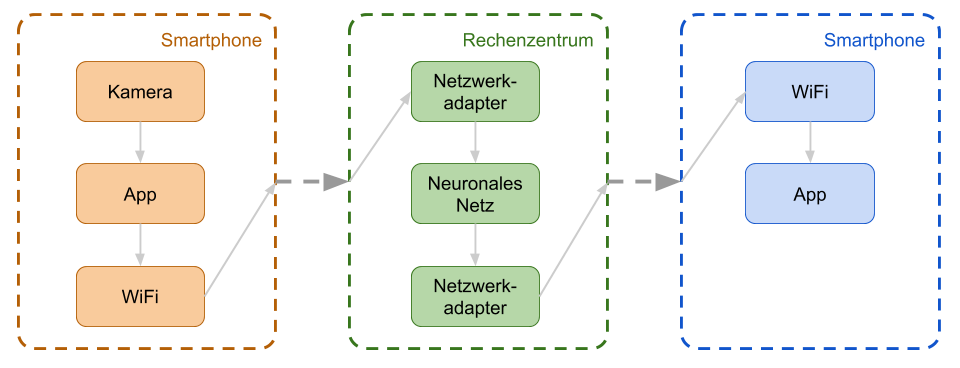
\includegraphics[width=1.00\textwidth]{BilderPDF/zielsetzung/App.png}
	\label{fig:App}
\end{figure}

Diese Anwendung ist nur exemplarisch und kein Teil der Umsetzung des Projektes.

\newpage

%%%%%%%%%%%%%%%%%%%%%%%%%%%%%%%%%%%%%%%%%%%%%%%%% Systeme %%%%%%%%%%%%%%%%%%%%%%%%%%%%%%%%%%%%%%%%%%%%%%%%%%%%%

\section*{\LARGE\textbf{Systeme}}

Im Zuge dieser Projektarbeit sollen verschiedene technische Realisierungen miteinander verglichen werden. Die relevanten Messdaten sind die Datenmenge gegen die benötigte Rechenzeit. Der Vergleich ist grundlegend auf vier verschiedene Hardwareplattformen beschränkt.


%%%%%%%%%%%%%%%%%%%%%%%%%%%%%%%%%%%%%%%%%%%%%%%%% CPU %%%%%%%%%%%%%%%%%%%%%%%%%%%%%%%%%%%%%%%%%%%%%%%%%%%%%

\section*{\LARGE\textbf{CPU}}

Die wohl simpelste Realisierung ist die Entwicklung einer regulären PC Anwendung. Diese lädt das Foto vom verfügbaren Massenspeicher und überträgt dieses an das in der Anwendung implementierte Neuronale Netz. Die Auswertung der Ausgangs Neuronen kann somit auch lokal geschehen. 

\begin{figure}[htbp]
	\centering
		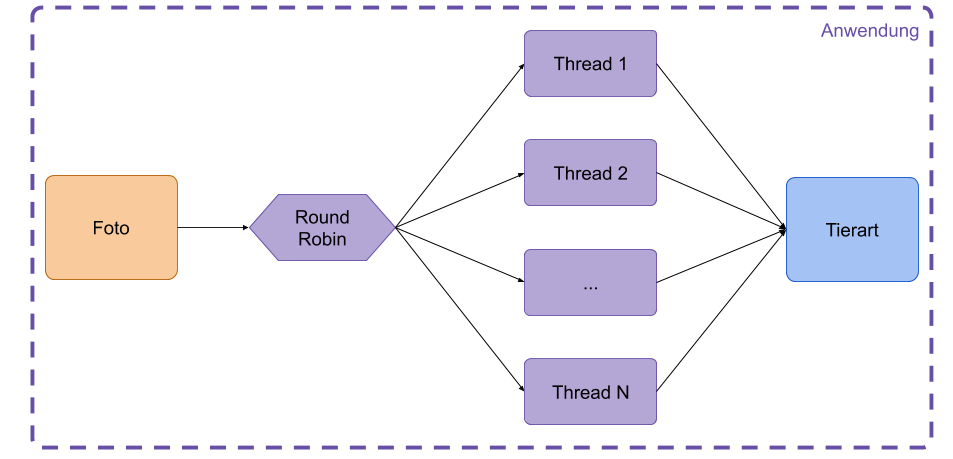
\includegraphics[width=1.00\textwidth]{BilderPDF/zielsetzung/System-PC.png}
	\label{fig:System-PC}
\end{figure}

Um ein möglichst gutes Ergebnis zu erzielen, muss die Anwendung mehrere CPU Kerne nutzen. Hierfür gilt, dass im Lernmodus das neuronale Netz in jeden Thread gespiegelt und anschließend zurück geschrieben werden muss, um die Parallelisierung gewährleisten zu können.\\

Um den Einfluss durch andere parallel laufende Anwendungen gering zu halten, ist es sinnvoll ein echtzeitfähiges Linux als Testsystem zu etablieren. Die Entwicklung kann auf beliebigen kompatiblen Plattformen geschehen.

\newpage

%%%%%%%%%%%%%%%%%%%%%%%%%%%%%%%%%%%%%%%%%%%%%%%%% FPGA %%%%%%%%%%%%%%%%%%%%%%%%%%%%%%%%%%%%%%%%%%%%%%%%%%%%%

\section*{\LARGE\textbf{FPGA}}

Eine weitere Möglichkeit ist die Anbindung eines FPGAs an die CPU. Dieser FPGA wäre dann hochspezialisiert auf die Ausführung des neuronalen Netzes zur Erkennung der Tiere. Dafür muss die CPU wie gehabt, das Bild von einem Massenspeicher laden und anschließend an den FPGA übertragen. Das übertragene Bild wird von dem FPGA ausgewertet und das Ergebnis der Auswertung zurück an die CPU übertragen. 

\begin{figure}[htbp]
	\centering
		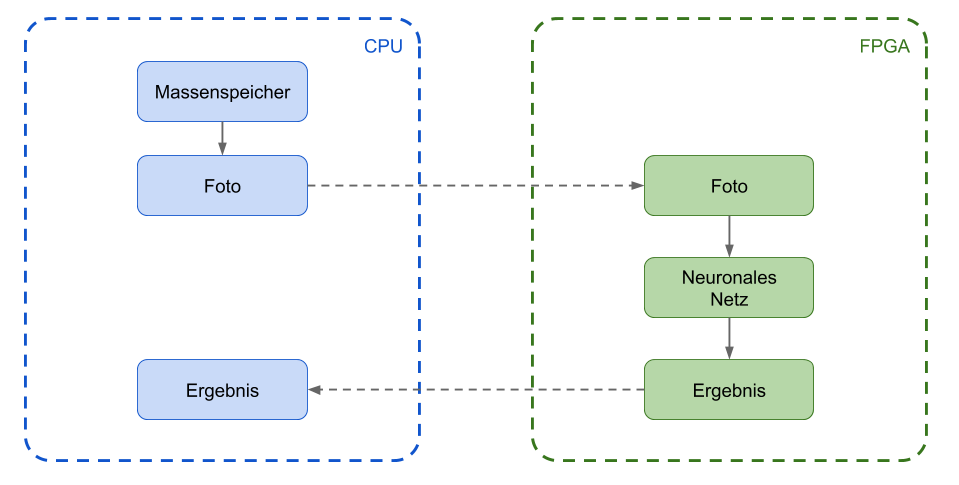
\includegraphics[width=1.00\textwidth]{BilderPDF/zielsetzung/System-FPGA.png}
	\label{fig:System-FPGA}
\end{figure}

\newpage

%%%%%%%%%%%%%%%%%%%%%%%%%%%%%%%%%%%%%%%%%%%%%%%%% TPU %%%%%%%%%%%%%%%%%%%%%%%%%%%%%%%%%%%%%%%%%%%%%%%%%%%%%

\section*{\LARGE\textbf{TPU}}

Der Vergleich wäre ohne aktuelle Domain Specific Architectures unvollständig. Daher soll dieser exemplarische Anwendungsfall auch auf einer Tensor Processing Unit (TPU) getestet werden. Auch hierfür wird das Foto des Tieres von der CPU von einem Massenspeicher geladen. Das geladene Foto wird an die TPU übertragen und von dieser verarbeitet. Die erhaltenen Resultate werden anschließend zur weiteren Verarbeitung an die CPU übermittelt.

\begin{figure}[htbp]
	\centering
		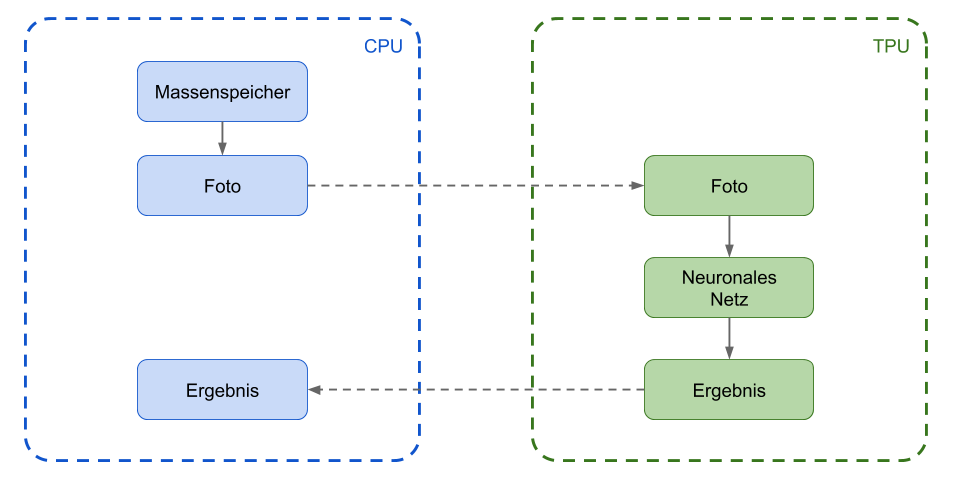
\includegraphics[width=1.00\textwidth]{BilderPDF/zielsetzung/System-TPU.png}
	\label{fig:System-TPU}
\end{figure}

\newpage

%%%%%%%%%%%%%%%%%%%%%%%%%%%%%%%%%%%%%%%%%%%%%%%%% GPU %%%%%%%%%%%%%%%%%%%%%%%%%%%%%%%%%%%%%%%%%%%%%%%%%%%%%

\section*{\LARGE\textbf{GPU}}

Im ersten Schritt ist es notwendig mittels CPU das Bild von dem Massenspeichergerät zu lesen. Im Anschluss wird das Bild von der CPU an die Grafikkarte über den verbundenen Bus übertragen. Nun berechnet das in der GPU befindliche neuronale Netz die Wahrscheinlichkeitswerte für alle definierten Tierarten. Nach Abschluss der Auswertung übermittelt die GPU das Ergebnis zurück an die CPU. Diese können dann weiter aufbereitet werden oder über eine entsprechende Schnittstelle weiter kommuniziert werden. 

\begin{figure}[htbp]
	\centering
		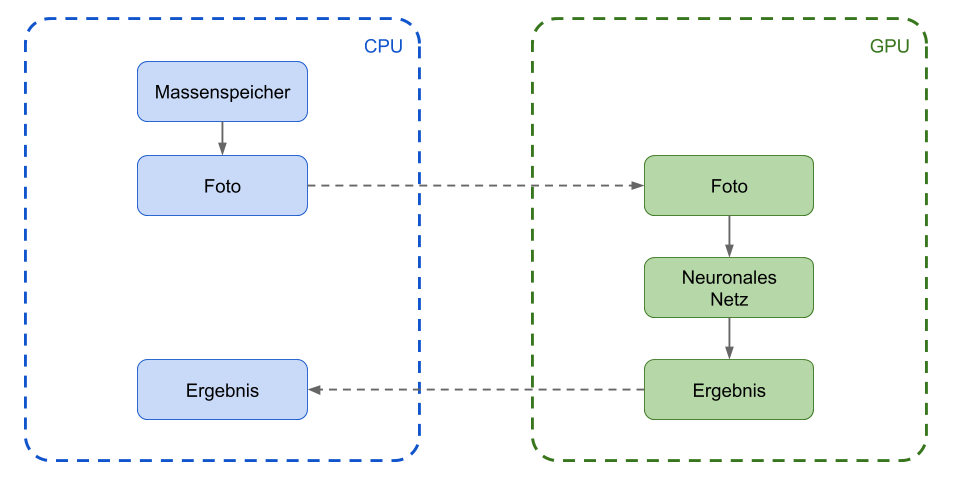
\includegraphics[width=1.00\textwidth]{BilderPDF/zielsetzung/System-GPU.png}
	\label{fig:System-GPU}
\end{figure}


Dies setzt eine Implementierung des neuronalen Netzes auf der GPU voraus.  

%%%%%%%%%%%%%%%%%%%%%%%%%%%%%%%%%%%%%%%%%%%%%%%%% Zeitmessung %%%%%%%%%%%%%%%%%%%%%%%%%%%%%%%%%%%%%%%%%%%%%%%%%%%%%

\section*{\LARGE\textbf{Zeitmessung}}

Die Messung der benötigten Zeit zur Auswertung ist ein essentieller Bestandteil des Projektes. Die Zeit wird für jedes System von der CPU gemessen. Die Zeitmessung beginnt ab dem Start der Übertragung des Fotos und endet mit dem vollständigen Empfang des Ergebnisses. Diese Zeitspanne ist per Definition die Auswertungszeit, welche die vollständige Bearbeitung des Auftrages enthält. Beginnend bei der Auftragserstellung (Start der Übertragung des Fotos) und dem Abschluss des Auftrages (Empfang der Ergebnisse). Dies ist für die Zeitmessung grob vereinfacht wie ein Funktionsaufruf aus Sicht der CPU,  genauer gesagt ein Remote Procedure Call (RPC). Der Beginn der Übertragung würde dann dem bereitstellen der Parameter entsprechen und das Erhalten der Ergebnisse wäre vergleichbar mit dem Rücksprung.

\newpage

%%%%%%%%%%%%%%%%%%%%%%%%%%%%%%%%%%%%%%%%%%%%%%%%% Kriterien %%%%%%%%%%%%%%%%%%%%%%%%%%%%%%%%%%%%%%%%%%%%%%%%%%%%%

\section*{\LARGE\textbf{Kriterien}}

\vspace{0.8cm}


\subsection*{\Large\textbf{Muss-Kriterien}}

\vspace{0.5cm}

\begin{itemize}
	\item Unterscheidung von mind. fünf verschiedenen Tierarten (Tiger, Elefant, Giraffe, Affe, Pinguin)
	\item Nach Abschluss des Projektes sind die Quellen Prof. Dr. Peter Gregorius permanent offen zu legen.
	\item Zu jedem System ist eine umfassende technische Dokumentation über das Konzept, den Systemaufbau und den groben Ablauf der Software zu erstellen.
\end{itemize}

\vspace{0.8cm}


\subsection*{\Large\textbf{Kann-Kriterien}}

\vspace{0.5cm}

\begin{itemize}
	\item In Abhängigkeit der verbleibenden Zeit, besteht die Möglichkeit der Unterstützung weiterer Tierarten (z.B. Vögel)
	\item Die Dokumentation des Quelltextes kann in ihrem Umfang durch die verbleibende Projektzeit variieren.
\end{itemize}

\vspace{0.8cm}


\subsection*{\Large\textbf{Ausschlusskriterien}}

\vspace{0.5cm}

\begin{itemize}
	\item Zu Gunsten der Realisierbarkeit innerhalb eines Semesters, werden nur Tierarten unterschieden, nicht aber Unterarten / Tierrassen. (Verringerte Komplexität)
	\item Um die Umsetzung innerhalb eines Semesters gewährleisten zu können, werden explizit verschiedenartige Tierarten gewählt, welche sich optisch nicht zu ähnlich sind. (Verringerter Trainingsaufwand)
	\item Es werden alle Bilder von Tieren ausgeschlossen, bei denen das Tier nicht das markanteste Element des Bildes ist. (Verringerter Trainingsaufwand)
	\item Das Beispiel der Zoo App, ist ausschließlich ein Beispiel. Die Umsetzung davon ist kein Bestandteil dieses Projektes
	\item Eine Gute Trefferquote beim Erkennen des Tieres wird nicht gewährleistet, da diese nicht im Vordergrund des Projektes steht. Im Vordergrund steht die reproduzierbaren Rechenoperationen um diese auf verschiedenen Plattformen durchzuführen.
	\item Die realisierten Lösungen müssen ausschließlich auf den in diesem Dokument definierten Plattformen lauffähig sein. 
\end{itemize}

\newpage

%%%%%%%%%%%%%%%%%%%%%%%%%%%%%%%%%%%%%%%%%%%%%%%%% Bildmaterial %%%%%%%%%%%%%%%%%%%%%%%%%%%%%%%%%%%%%%%%%%%%%%%%%%%%%

\section*{\LARGE\textbf{Bildmaterial}}

Im folgenden sind exemplarisch Bilder aufgeführt, die für die Auswertung zulässig bzw. unzulässig wären. \\

\textbf{Zulässig:}

\begin{figure}[htbp]
	\centering
		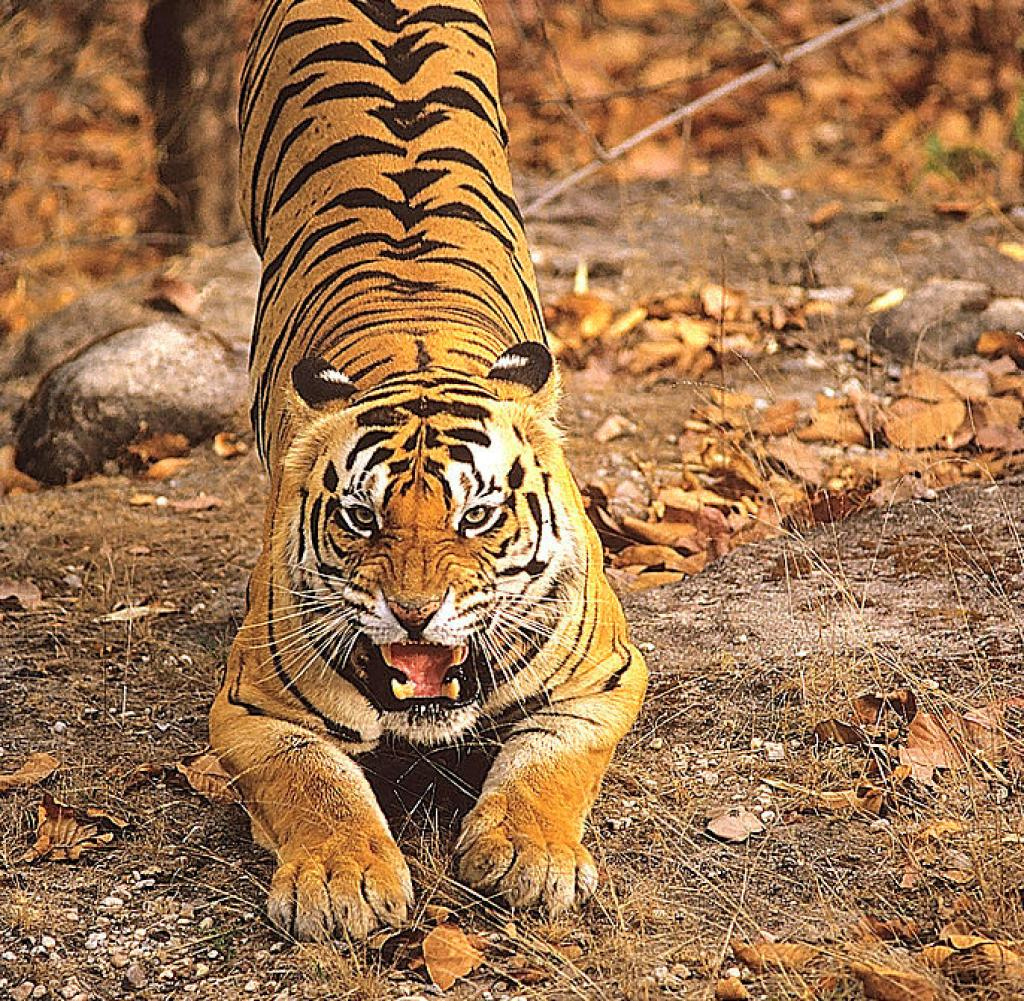
\includegraphics[width=0.50\textwidth]{BilderPDF/zielsetzung/tiger_01.jpg}
	\caption{Tiger im Laub \cite{tiger_laub}}
	\label{fig:tiger_01}
\end{figure}

\vspace{0.5cm}

\begin{figure}[htbp]
	\centering
		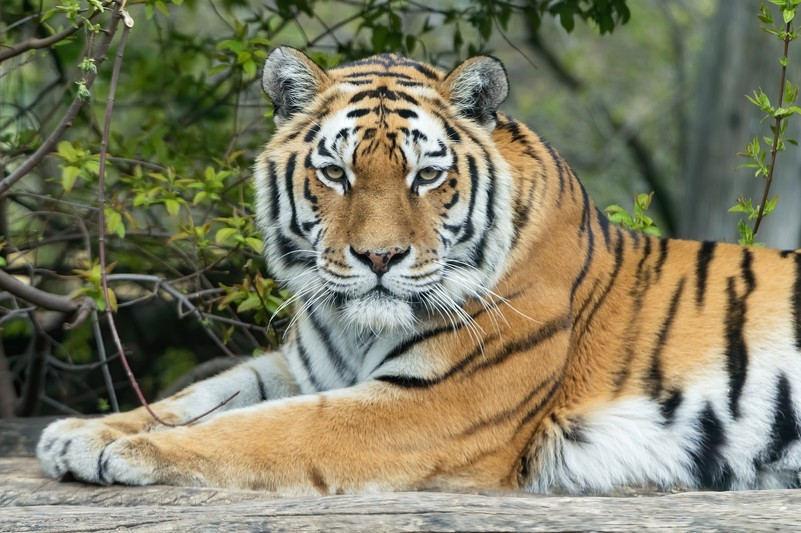
\includegraphics[width=0.60\textwidth]{BilderPDF/zielsetzung/tiger_02.jpg}
	\caption{Tiger liegt auf einem Stein \cite{tiger_stein}}
	\label{fig:tiger_02}
\end{figure}

\newpage

\begin{figure}[htbp]
	\centering
		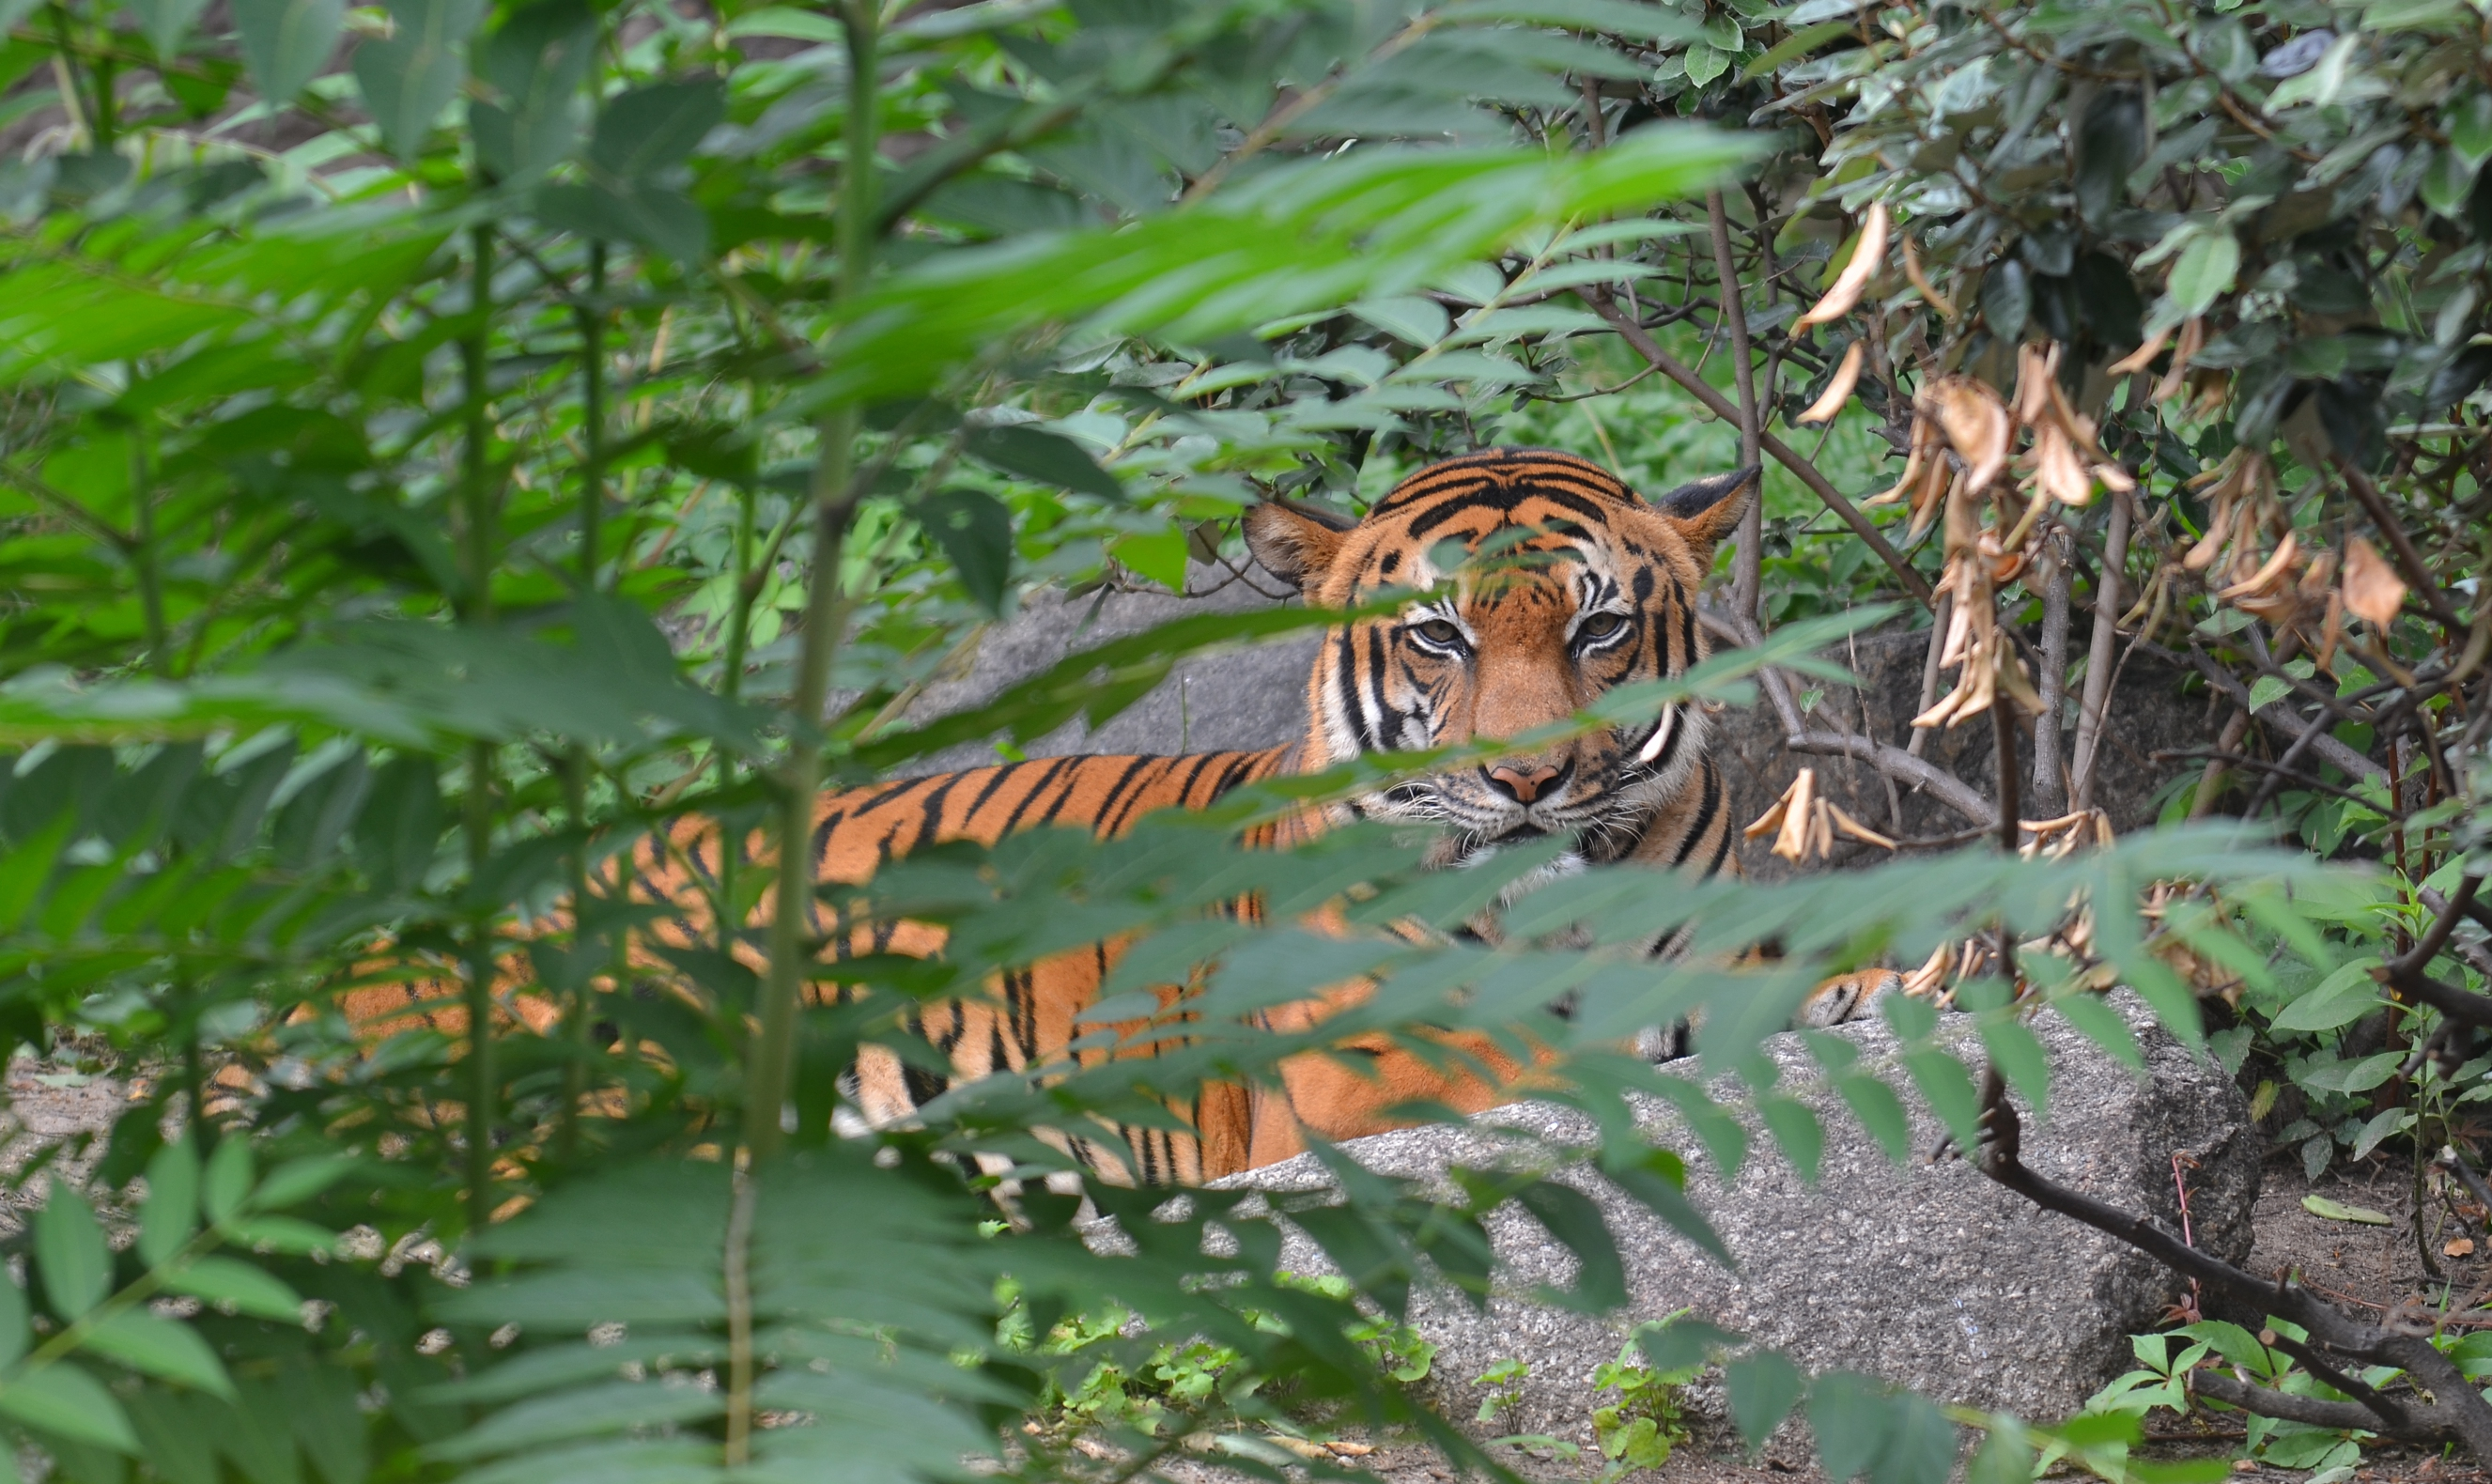
\includegraphics[width=0.60\textwidth]{BilderPDF/zielsetzung/tiger_03.jpg}
	\caption{Tiger leicht verdeckt \cite{tiger_leicht_verdeckt}}
	\label{fig:tiger_03}
\end{figure}

\vspace{5cm}

\textbf{Unzulässig:}

\begin{figure}[htbp]
	\centering
		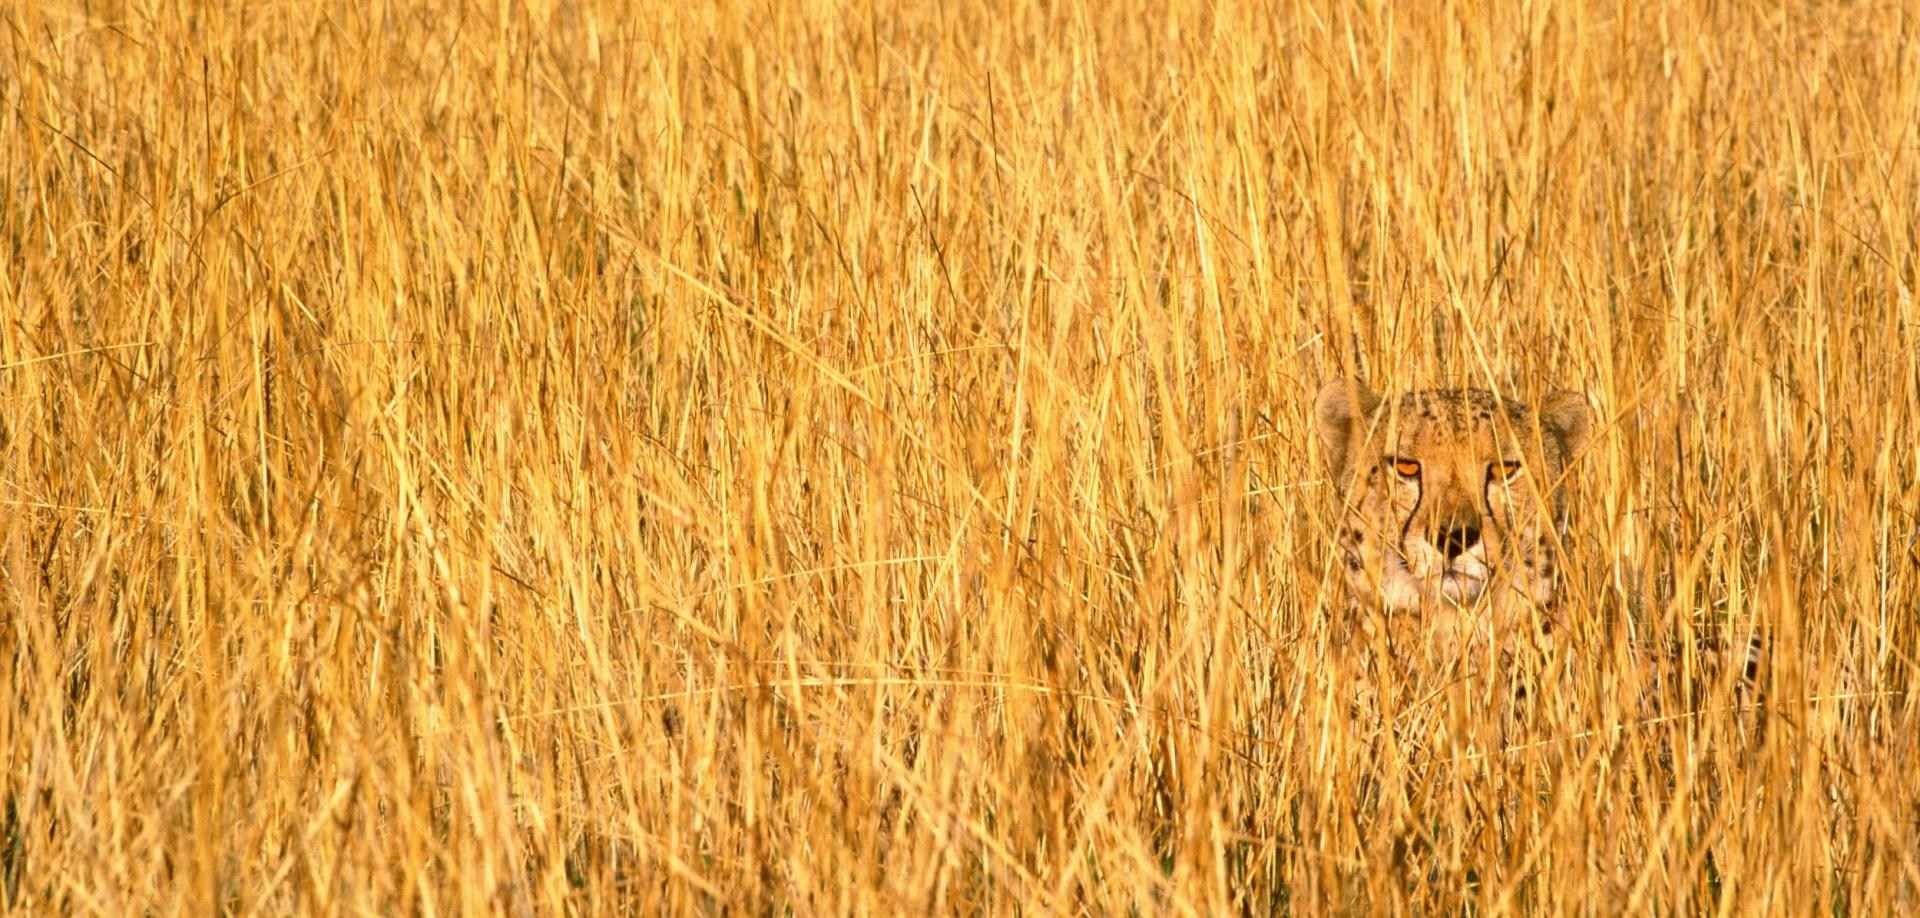
\includegraphics[width=0.60\textwidth]{BilderPDF/zielsetzung/tiger_04.jpg}
	\caption{Tiger verdeckt \cite{tiger_verdeckt}}
	\label{fig:tiger_04}
\end{figure}